% pipeline_variant_a.tex — pipeline: geometry → noise → performance
\documentclass[tikz,border=8pt]{standalone}

\usepackage{amsmath,amssymb,bm}
\usepackage{tikz}
\usetikzlibrary{arrows.meta,calc,positioning,fit,backgrounds,
                decorations.pathreplacing,shapes.geometric,quotes}

\definecolor{okBlue}{HTML}{4472C4}
\definecolor{okRed}{HTML}{C0504D}
\definecolor{okGreen}{HTML}{55A868}
\definecolor{okOrange}{HTML}{D98E04}
\definecolor{softBlue}{HTML}{EAF1FB}
\definecolor{softGreen}{HTML}{EDF7F0}

\tikzset{
  >={Latex[length=2.4mm,width=2.2mm]},
  every node/.style={font=\normalsize},
  mathbox/.style={draw=black!55, rounded corners=2.5pt, very thick,
                  fill=black!2, inner sep=6pt, align=center},
  panel/.style={draw=black!55, rounded corners=2.5pt, line width=0.8pt,
                fill=white},
  flow/.style={-{Latex[length=2.5mm]}, line width=1.1pt, draw=black!70},
  thinflow/.style={-{Latex[length=2.0mm]}, line width=0.9pt, draw=black!55},
  faintcol/.style={draw=black!18, line width=0.6pt},
  crossdot/.style={diamond, draw=okOrange!80!black, fill=okOrange!85,
                   minimum size=6pt, inner sep=0pt},
  qz/.style={diamond, draw=okOrange!85!black, fill=white,
             minimum size=5.5pt, inner sep=0pt, line width=0.7pt},
  routeA/.style={draw=okBlue!85!black, line width=1.2pt,
                 line cap=round, line join=round},
  routeB/.style={draw=okRed!85!black, line width=1.2pt,
                 line cap=round, line join=round},
  layA/.style={draw=okBlue!55!black, fill=okBlue!10, line width=0.7pt},
  layB/.style={draw=okRed!55!black, fill=okRed!10, line width=0.7pt},
  layBase/.style={draw=black!35, fill=black!5, line width=0.7pt},
  titleline/.style={font=\normalsize\bfseries},
  branchchip/.style={draw=black!45, rounded corners=2pt, inner sep=5pt,
                     align=center, font=\normalsize},
}

\begin{document}
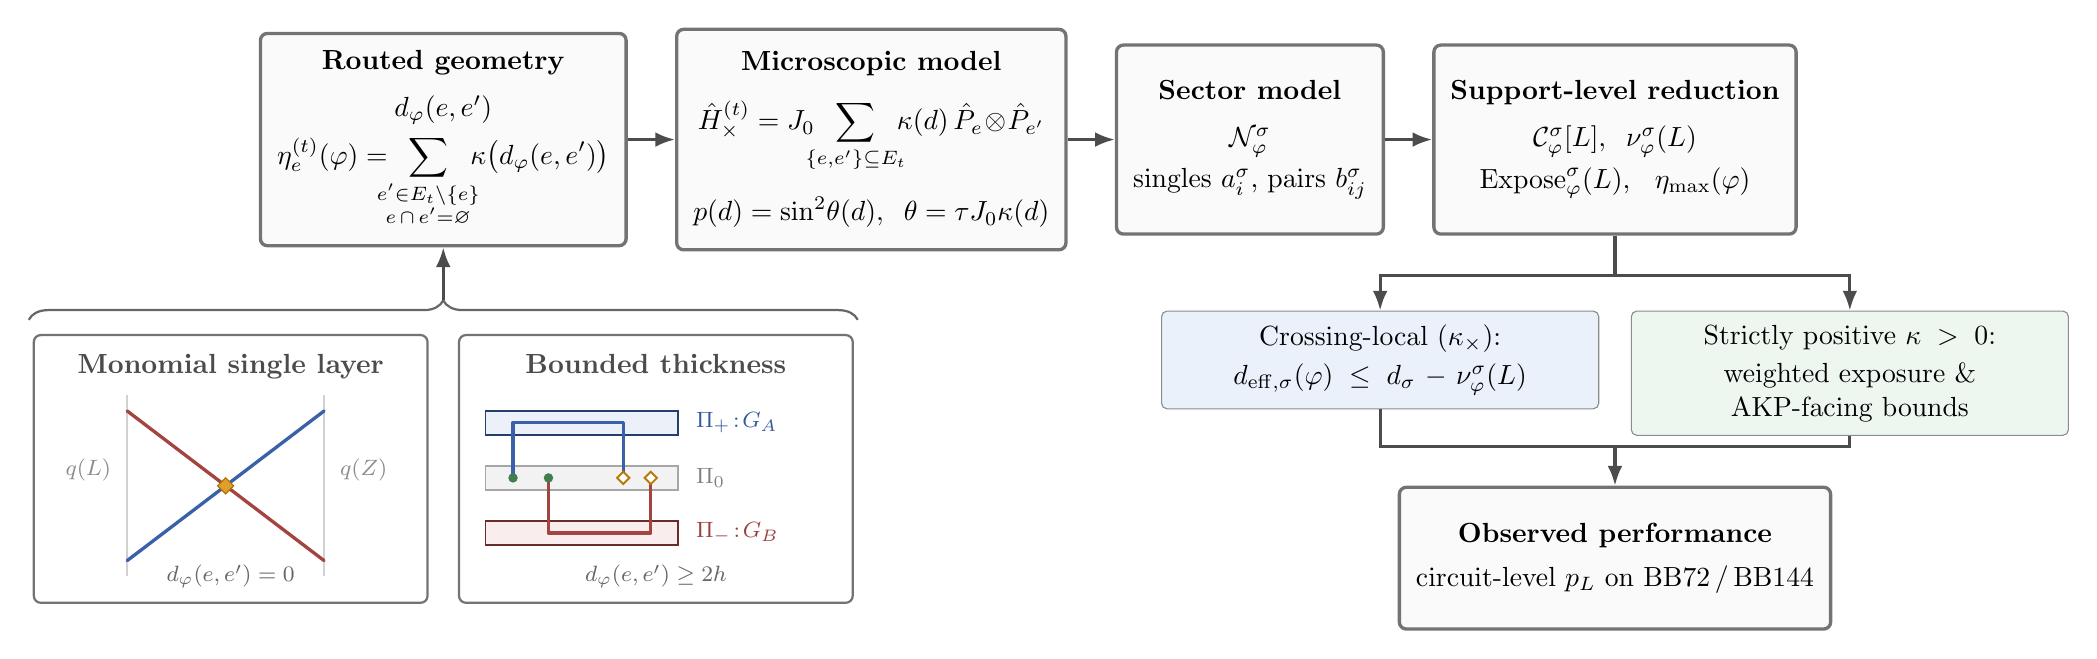
\begin{tikzpicture}[x=1cm, y=1cm]

% ====================================================================
% HORIZONTAL PIPELINE (top row, 4 boxes)
% ====================================================================
\node[mathbox, minimum width=3.6cm, minimum height=2.4cm,
      anchor=west] (geo) at (0,0)
  {\textbf{Routed geometry}\\[5pt]
   $d_{\varphi}(e,e')$\\[3pt]
   $\displaystyle\eta_{e}^{(t)}(\varphi)
    =\!\!\!\!\sum_{\substack{e'\in E_t\setminus\{e\}\\e\,\cap\, e'=\varnothing}}
    \!\!\!\kappa\bigl(d_{\varphi}(e,e')\bigr)$};

\node[mathbox, minimum width=3.8cm, minimum height=2.8cm,
      anchor=west] (micro) at ($(geo.east)+(0.60,0)$)
  {\textbf{Microscopic model}\\[8pt]
   $\displaystyle\hat{H}_{\times}^{(t)}
    = J_0\!\!\!\sum_{\{e,e'\}\subseteq E_t}\!\!\!
    \kappa(d)\,\hat{P}_e\!\otimes\!\hat{P}_{e'}$\\[8pt]
   $p(d)=\sin^{2}\!\theta(d),\;\;\theta=\tau J_0\kappa(d)$};

\node[mathbox, minimum width=3.0cm, minimum height=2.4cm,
      anchor=west] (sector) at ($(micro.east)+(0.60,0)$)
  {\textbf{Sector model}\\[5pt]
   $\mathcal{N}_{\varphi}^{\sigma}$\\[3pt]
   singles $a_i^{\sigma}$, pairs $b_{ij}^{\sigma}$};

\node[mathbox, minimum width=3.8cm, minimum height=2.4cm,
      anchor=west] (graph) at ($(sector.east)+(0.60,0)$)
  {\textbf{Support-level reduction}\\[5pt]
   $\mathcal{C}_{\varphi}^{\sigma}[L],\;\;
    \nu_{\varphi}^{\sigma}(L)$\\[3pt]
   $\mathrm{Expose}_{\varphi}^{\sigma}(L)$,\;\;
    $\eta_{\max}(\varphi)$};

% Horizontal pipeline arrows
\foreach \a/\b in {geo/micro, micro/sector, sector/graph}{
  \draw[flow] (\a.east) -- (\b.west);
}

% ====================================================================
% EMBEDDING PANELS (below geo, side by side — input to pipeline)
% ====================================================================

% ── Monomial single layer (left) ─────────────────────────────────
\node[panel, minimum width=5.0cm, minimum height=3.4cm,
      anchor=north] (mono) at ($(geo.south)+(-2.70,-1.10)$) {};

\node[titleline, anchor=north, text=black!70]
  at ($(mono.north)+(0,-0.14)$) {Monomial single layer};

% Guide lines — symmetric excess (0.20) above and below crossing endpoints
\draw[faintcol] ($(mono.south west)+(1.20,0.35)$)
             -- ($(mono.south west)+(1.20,2.65)$);
\draw[faintcol] ($(mono.south west)+(3.70,0.35)$)
             -- ($(mono.south west)+(3.70,2.65)$);

% q(L) and q(Z) labels
\node[font=\footnotesize, text=black!45, anchor=east]
  at ($(mono.south west)+(1.12,1.70)$) {$q(L)$};
\node[font=\footnotesize, text=black!45, anchor=west]
  at ($(mono.south west)+(3.78,1.70)$) {$q(Z)$};

% Crossing edges
\draw[routeA] ($(mono.south west)+(1.20,0.55)$)
           -- ($(mono.south west)+(3.70,2.45)$);
\draw[routeB] ($(mono.south west)+(1.20,2.45)$)
           -- ($(mono.south west)+(3.70,0.55)$);
\node[crossdot] at ($(mono.south west)+(2.45,1.50)$) {};

% Bottom label
\node[font=\footnotesize, text=black!60, anchor=south]
  at ($(mono.south)+(0,0.08)$) {$d_\varphi(e,e')=0$};

% ── Bounded thickness (right) ────────────────────────────────────
\node[panel, minimum width=5.0cm, minimum height=3.4cm,
      anchor=north] (bi) at ($(geo.south)+(+2.70,-1.10)$) {};

\node[titleline, anchor=north, text=black!70]
  at ($(bi.north)+(0,-0.14)$) {Bounded thickness};

% Three slabs
\fill[layA]    ($(bi.south west)+(0.35,2.15)$)
     rectangle ($(bi.south west)+(2.80,2.45)$);
\fill[layBase] ($(bi.south west)+(0.35,1.45)$)
     rectangle ($(bi.south west)+(2.80,1.75)$);
\fill[layB]    ($(bi.south west)+(0.35,0.75)$)
     rectangle ($(bi.south west)+(2.80,1.05)$);

% Slab labels
\node[anchor=west, font=\footnotesize, text=okBlue!80!black]
  at ($(bi.south west)+(2.90,2.30)$) {$\Pi_{+}\!:\!G_A$};
\node[anchor=west, font=\footnotesize, text=black!50]
  at ($(bi.south west)+(2.90,1.60)$) {$\Pi_{0}$};
\node[anchor=west, font=\footnotesize, text=okRed!80!black]
  at ($(bi.south west)+(2.90,0.90)$) {$\Pi_{-}\!:\!G_B$};

% Routes
\draw[routeA]
  ($(bi.south west)+(0.70,1.60)$) -- ($(bi.south west)+(0.70,2.30)$)
  -- ($(bi.south west)+(2.10,2.30)$) -- ($(bi.south west)+(2.10,1.60)$);
\draw[routeB]
  ($(bi.south west)+(1.15,1.60)$) -- ($(bi.south west)+(1.15,0.90)$)
  -- ($(bi.south west)+(2.45,0.90)$) -- ($(bi.south west)+(2.45,1.60)$);

% Endpoint markers
\fill[okGreen!75!black] ($(bi.south west)+(0.70,1.60)$) circle (0.06);
\fill[okGreen!75!black] ($(bi.south west)+(1.15,1.60)$) circle (0.06);
\node[qz, scale=0.85] at ($(bi.south west)+(2.10,1.60)$) {};
\node[qz, scale=0.85] at ($(bi.south west)+(2.45,1.60)$) {};

% Bottom label
\node[font=\footnotesize, text=black!60, anchor=south]
  at ($(bi.south)+(0,0.08)$) {$d_\varphi(e,e')\ge 2h$};

% ── Horizontal brace above panels, arrow up to geo ───────────────
\draw[decorate, decoration={brace, amplitude=7pt},
      draw=black!60, line width=0.8pt]
  ($(mono.north west)+(-0.05,0.18)$) -- ($(bi.north east)+(0.05,0.18)$)
  coordinate[midway] (bracemid);

% Arrow starts at brace tip (bracemid + amplitude ≈ 0.25cm)
\draw[flow] ($(bracemid)+(0,0.25)$) -- (geo.south);

% ====================================================================
% VERTICAL from graph: fork → two chips side by side → obs
% ====================================================================
\draw[line width=1.1pt, draw=black!70]
  (graph.south) -- ++(0,-0.50) coordinate (fork);

\node[branchchip, fill=softBlue, text width=5.2cm,
      anchor=north east] (cross) at ($(fork)+(-0.20,-0.45)$)
  {Crossing-local ($\kappa_{\times}$):\\[2pt]
   $d_{\mathrm{eff},\sigma}(\varphi)
    \le d_\sigma - \nu_{\varphi}^{\sigma}(L)$};

\node[branchchip, fill=softGreen, text width=5.2cm,
      anchor=north west] (expo) at ($(fork)+(0.20,-0.45)$)
  {Strictly positive $\kappa > 0$:\\[2pt]
   weighted exposure \& AKP-facing bounds};

% Fork → chips (uniform flow style)
\coordinate (crossAbove) at ($(cross.north)+(0,0.15)$);
\coordinate (expoAbove)  at ($(expo.north)+(0,0.15)$);
\draw[line width=1.1pt, draw=black!70]
  (fork) -| (crossAbove);
\draw[flow] (crossAbove) -- (cross.north);
\draw[line width=1.1pt, draw=black!70]
  (fork) -| (expoAbove);
\draw[flow] (expoAbove) -- (expo.north);

% Observed performance below the two chips
\node[mathbox, minimum width=5.0cm, minimum height=1.8cm,
      anchor=north] (obs) at ($(cross.south)!0.5!(expo.south)+(0,-0.80)$)
  {\textbf{Observed performance}\\[4pt]
   circuit-level $p_L$ on BB72\,/\,BB144};

% Chips → obs: merge pattern (inverted fork, uniform flow style)
\coordinate (merge) at ($(obs.north)+(0,0.50)$);
\draw[line width=1.1pt, draw=black!70]
  (cross.south) |- (merge);
\draw[line width=1.1pt, draw=black!70]
  (expo.south) |- (merge);
\draw[flow] (merge) -- (obs.north);

\end{tikzpicture}
\end{document}
